\section{Decision trees}

\begin{enumerate}
\item Concrete sample training data.
\begin{enumerate}
\item The sample entropy $H(Y)$ is 0.985. \begin{align*}
H(Y)= & \;-\sum_{y}p(Y=y)log_{2}p(Y=y)\\
= & \;-p(Y=+)log_{2}p(Y=+)-p(Y=-)log_{2}p(Y=-)\\
= & \;\frac{4}{7}log_{2}(\frac{7}{4})+\frac{3}{7}log_{2}(\frac{7}{3})\\
= & \;0.985\end{align*}

\item The information gains are $IG(X_{1})=0.183$ and $IG(X_{2})=0.045$.
\begin{align*}
IG(X_{1})= & \; H(Y)-H(Y|X_{1})\\
= & \; H(Y)+\sum_{y,x}p(Y=y,X_{1}=x)log_{2}p(Y=y|X_{1}=x)\\
= & \; H(Y)+\sum_{y,x}p(Y=y,X_{1}=x)log_{2}\frac{p(Y=y,X_{1}=x)}{p(X_{1}=x)}\\
= & \;0.985+\frac{1}{3}log_{2}\frac{7}{8}+\frac{5}{21}log_{2}\frac{5}{13}+\frac{1}{21}log_{2}\frac{1}{8}+\frac{8}{21}log_{2}\frac{8}{13}\\
= & \;0.183\\
IG(X_{2})= & \; H(Y)-H(Y|X_{2})\\
= & \; H(Y)+\sum_{y,x}p(Y=y,X_{2}=x)log_{2}p(Y=y|X_{2}=x)\\
= & \;0.985+\frac{1}{3}log_{2}\frac{7}{10}+\frac{5}{21}log_{2}\frac{5}{11}+\frac{1}{7}log_{2}\frac{3}{10}+\frac{2}{7}log_{2}\frac{6}{11}\\
= & \;0.045\end{align*}


  \item The decision tree that would be learned is shown in Figure
    \ref{fig:decision_tree}.
    %% The [H], in combination with the float package, forces latex to
    %% generate the figure in exactly this part of the document
    %% instead of ``floating'' it to another part.
    \begin{figure}[H]
      \centering
      \tikzstyle{dir}=[->, very thick]
      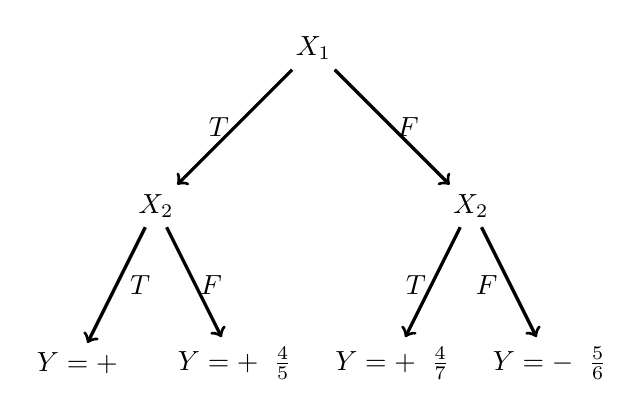
\begin{tikzpicture}[auto]
        \node[rectangle] (X1) at (0,0) {$X_1$};
        \node (X20) at (-2,-2) {$X_2$};
        \node (X21) at (2,-2) {$X_2$};
	\node (leaf1) at (-3,-4) {$Y=+$};
	\node (leaf2) at (-1,-4) {$Y=+\;\;\frac{4}{5}$};
	\node (leaf3) at (1,-4) {$Y=+\;\;\frac{4}{7}$};
	\node (leaf4) at (3,-4) {$Y=-\;\; \frac{5}{6}$};

        \draw[dir] (X1) to [above] node {} (X20);
        \draw[dir] (X1) to [above] node {} (X21);
	\draw[dir] (X20) to [above] node {} (leaf1);
	\draw[dir] (X20) to [above] node {} (leaf2);
	\draw[dir] (X21) to [above] node {} (leaf3);
	\draw[dir] (X21) to [above] node {} (leaf4);
	\node (label1) at (-1.2,-1) {$T$};
	\node (label2) at (1.2,-1) {$F$};
	\node (label3) at (-2.2,-3) {$T$};
	\node (label4) at (-1.3,-3) {$F$};
	\node (label5) at (1.3,-3) {$T$};
	\node (label6) at (2.2,-3) {$F$};
	
      \end{tikzpicture}
      \caption{The decision tree that would be learned.}
      \label{fig:decision_tree}
    \end{figure}
  \end{enumerate}

\item Proof that $IG(x,y)=H[x]-H[x\mid y]=H[y]-H[y\mid x]$, starting from
the definition in terms of KL-divergence: \begin{align*}
IG(x,y)= & \; KL\left(p(x,y)||p(x)p(y)\right)\\
= & \;\sum_{x}\sum_{y}p(x,y)log(\frac{p(x)p(y)}{p(x,y)})\\
= & \;\sum_{x}\sum_{y}p(x,y)logp(x)-\sum_{x}\sum_{y}p(x,y)logp(x|y)\\
= & \;\sum_{x}p(x)logp(x)-\sum_{x}\sum_{y}p(x,y)logp(x|y)\\
= & \; H[x]-H[x\mid y]\end{align*}
\end{enumerate}
